% Created by tikzDevice version 0.12 on 2019-01-18 11:36:19
% !TEX encoding = UTF-8 Unicode
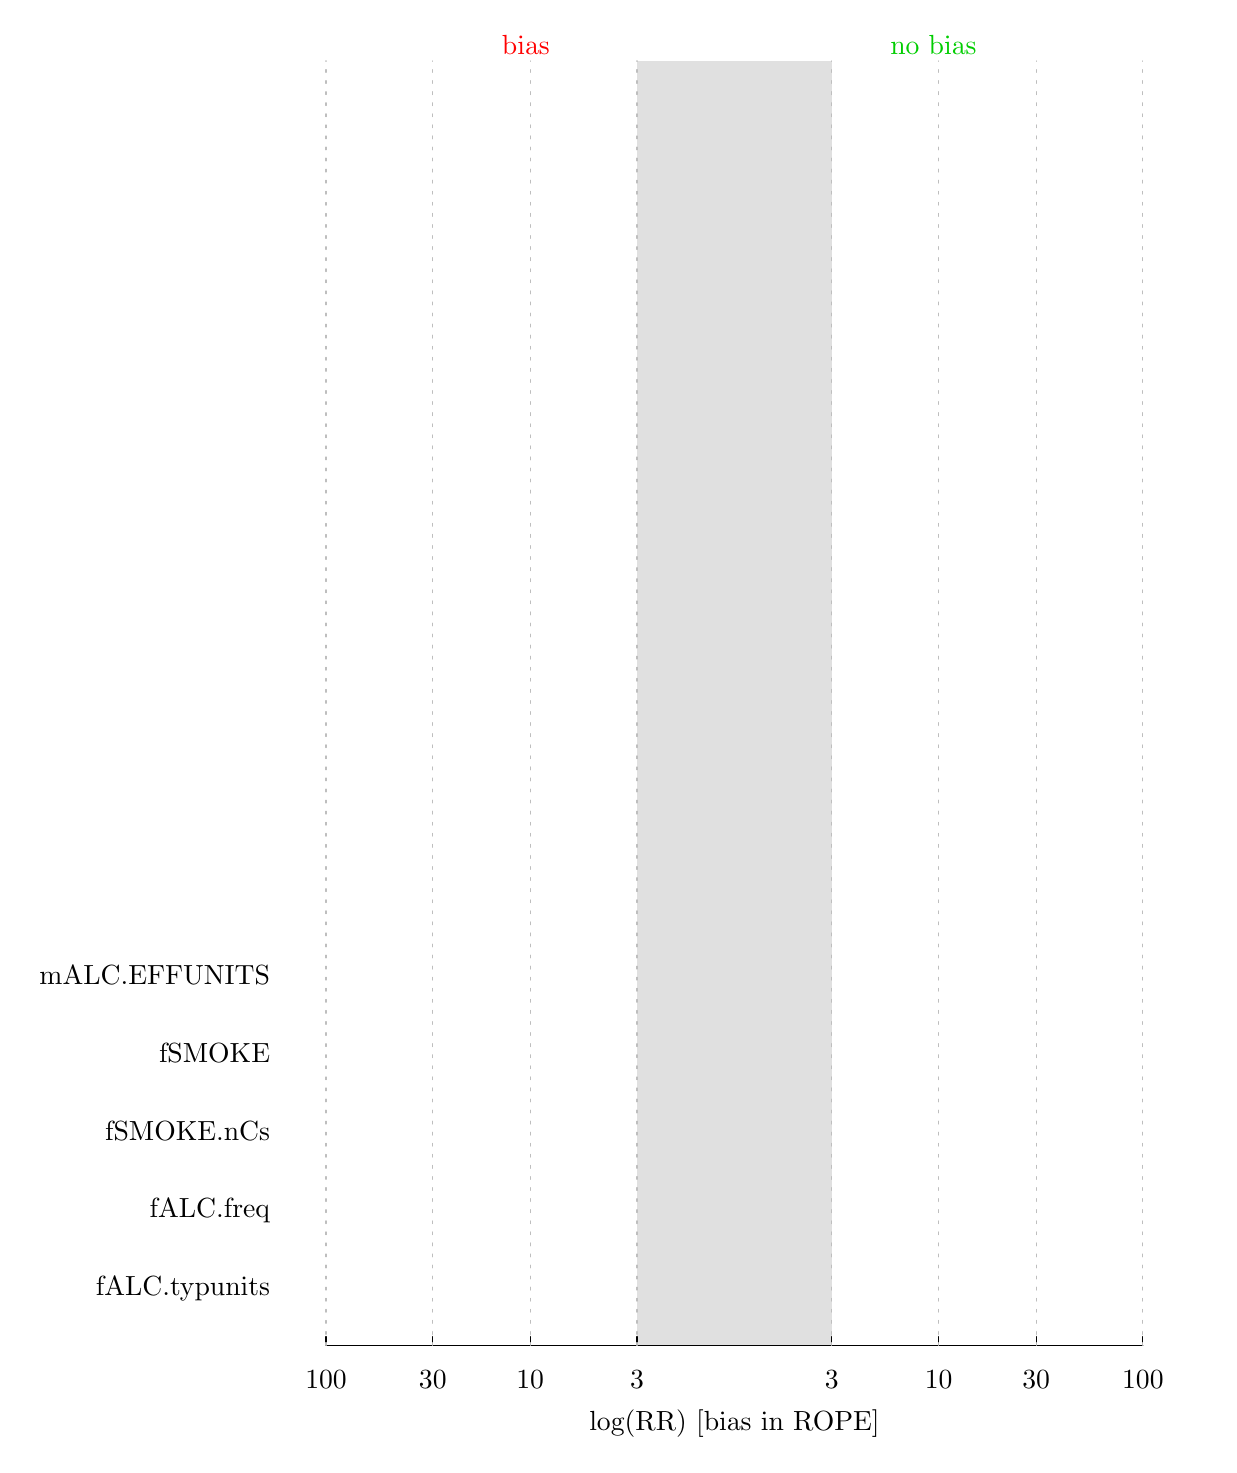
\begin{tikzpicture}[x=1pt,y=1pt]
\definecolor{fillColor}{RGB}{255,255,255}
\path[use as bounding box,fill=fillColor,fill opacity=0.00] (0,0) rectangle (426.79,512.15);
\begin{scope}
\path[clip] (  0.00,  0.00) rectangle (426.79,512.15);
\definecolor{drawColor}{RGB}{0,0,0}

\node[text=drawColor,anchor=base,inner sep=0pt, outer sep=0pt, scale=  1.00] at (255.40,  5.40) {log(RR) [bias in ROPE]};
\end{scope}
\begin{scope}
\path[clip] ( 96.00, 36.00) rectangle (414.79,500.15);
\definecolor{fillColor}{gray}{0.88}

\path[fill=fillColor] (220.19, 36.00) rectangle (290.60,500.15);
\end{scope}
\begin{scope}
\path[clip] (  0.00,  0.00) rectangle (426.79,512.15);
\definecolor{drawColor}{RGB}{0,0,0}

\path[draw=drawColor,line width= 0.4pt,line join=round,line cap=round] (107.81, 36.00) -- (402.98, 36.00);

\path[draw=drawColor,line width= 0.4pt,line join=round,line cap=round] (107.81, 36.00) -- (107.81, 39.19);

\path[draw=drawColor,line width= 0.4pt,line join=round,line cap=round] (146.39, 36.00) -- (146.39, 39.19);

\path[draw=drawColor,line width= 0.4pt,line join=round,line cap=round] (181.60, 36.00) -- (181.60, 39.19);

\path[draw=drawColor,line width= 0.4pt,line join=round,line cap=round] (220.19, 36.00) -- (220.19, 39.19);

\path[draw=drawColor,line width= 0.4pt,line join=round,line cap=round] (290.60, 36.00) -- (290.60, 39.19);

\path[draw=drawColor,line width= 0.4pt,line join=round,line cap=round] (329.19, 36.00) -- (329.19, 39.19);

\path[draw=drawColor,line width= 0.4pt,line join=round,line cap=round] (364.40, 36.00) -- (364.40, 39.19);

\path[draw=drawColor,line width= 0.4pt,line join=round,line cap=round] (402.98, 36.00) -- (402.98, 39.19);

\node[text=drawColor,anchor=base,inner sep=0pt, outer sep=0pt, scale=  1.00] at (107.81, 20.40) {100};

\node[text=drawColor,anchor=base,inner sep=0pt, outer sep=0pt, scale=  1.00] at (146.39, 20.40) {30};

\node[text=drawColor,anchor=base,inner sep=0pt, outer sep=0pt, scale=  1.00] at (181.60, 20.40) {10};

\node[text=drawColor,anchor=base,inner sep=0pt, outer sep=0pt, scale=  1.00] at (220.19, 20.40) {3};

\node[text=drawColor,anchor=base,inner sep=0pt, outer sep=0pt, scale=  1.00] at (290.60, 20.40) {3};

\node[text=drawColor,anchor=base,inner sep=0pt, outer sep=0pt, scale=  1.00] at (329.19, 20.40) {10};

\node[text=drawColor,anchor=base,inner sep=0pt, outer sep=0pt, scale=  1.00] at (364.40, 20.40) {30};

\node[text=drawColor,anchor=base,inner sep=0pt, outer sep=0pt, scale=  1.00] at (402.98, 20.40) {100};
\end{scope}
\begin{scope}
\path[clip] ( 96.00, 36.00) rectangle (414.79,500.15);
\definecolor{drawColor}{RGB}{190,190,190}

\path[draw=drawColor,line width= 0.4pt,dash pattern=on 1pt off 3pt ,line join=round,line cap=round] (107.81, 36.00) -- (107.81,500.15);

\path[draw=drawColor,line width= 0.4pt,dash pattern=on 1pt off 3pt ,line join=round,line cap=round] (146.39, 36.00) -- (146.39,500.15);

\path[draw=drawColor,line width= 0.4pt,dash pattern=on 1pt off 3pt ,line join=round,line cap=round] (181.60, 36.00) -- (181.60,500.15);

\path[draw=drawColor,line width= 0.4pt,dash pattern=on 1pt off 3pt ,line join=round,line cap=round] (220.19, 36.00) -- (220.19,500.15);

\path[draw=drawColor,line width= 0.4pt,dash pattern=on 1pt off 3pt ,line join=round,line cap=round] (290.60, 36.00) -- (290.60,500.15);

\path[draw=drawColor,line width= 0.4pt,dash pattern=on 1pt off 3pt ,line join=round,line cap=round] (329.19, 36.00) -- (329.19,500.15);

\path[draw=drawColor,line width= 0.4pt,dash pattern=on 1pt off 3pt ,line join=round,line cap=round] (364.40, 36.00) -- (364.40,500.15);

\path[draw=drawColor,line width= 0.4pt,dash pattern=on 1pt off 3pt ,line join=round,line cap=round] (402.98, 36.00) -- (402.98,500.15);
\end{scope}
\begin{scope}
\path[clip] (  0.00,  0.00) rectangle (426.79,512.15);
\definecolor{drawColor}{RGB}{255,0,0}

\node[text=drawColor,anchor=base,inner sep=0pt, outer sep=0pt, scale=  1.00] at (180.02,502.55) {bias};
\definecolor{drawColor}{RGB}{0,205,0}

\node[text=drawColor,anchor=base east,inner sep=0pt, outer sep=0pt, scale=  1.00] at (342.88,502.55) {no bias};
\definecolor{drawColor}{RGB}{0,0,0}

\node[text=drawColor,anchor=base east,inner sep=0pt, outer sep=0pt, scale=  1.00] at ( 87.60, 53.96) {fALC.typunits};

\node[text=drawColor,anchor=base east,inner sep=0pt, outer sep=0pt, scale=  1.00] at ( 87.60, 82.05) {fALC.freq};

\node[text=drawColor,anchor=base east,inner sep=0pt, outer sep=0pt, scale=  1.00] at ( 87.60,110.14) {fSMOKE.nCs};

\node[text=drawColor,anchor=base east,inner sep=0pt, outer sep=0pt, scale=  1.00] at ( 87.60,138.23) {fSMOKE};

\node[text=drawColor,anchor=base east,inner sep=0pt, outer sep=0pt, scale=  1.00] at ( 87.60,166.32) {mALC.EFFUNITS};
\end{scope}
\end{tikzpicture}
\begin{tikzpicture}[x=1pt,y=1pt]
\definecolor{fillColor}{RGB}{255,255,255}
\path[use as bounding box,fill=fillColor,fill opacity=0.00] (0,0) rectangle (426.79,512.15);
\begin{scope}
\path[clip] (  0.00,  0.00) rectangle (426.79,512.15);
\definecolor{drawColor}{RGB}{0,0,0}

\path[draw=drawColor,line width= 0.4pt,line join=round,line cap=round] (163.15, 36.00) -- (347.64, 36.00);

\path[draw=drawColor,line width= 0.4pt,line join=round,line cap=round] (163.15, 36.00) -- (163.15, 39.19);

\path[draw=drawColor,line width= 0.4pt,line join=round,line cap=round] (255.40, 36.00) -- (255.40, 39.19);

\path[draw=drawColor,line width= 0.4pt,line join=round,line cap=round] (347.64, 36.00) -- (347.64, 39.19);

\node[text=drawColor,anchor=base,inner sep=0pt, outer sep=0pt, scale=  1.00] at (163.15, 18.00) {-5};

\node[text=drawColor,anchor=base,inner sep=0pt, outer sep=0pt, scale=  1.00] at (255.40, 18.00) {0};

\node[text=drawColor,anchor=base,inner sep=0pt, outer sep=0pt, scale=  1.00] at (347.64, 18.00) {5};
\end{scope}
\begin{scope}
\path[clip] (  0.00,  0.00) rectangle (426.79,512.15);
\definecolor{drawColor}{RGB}{0,0,0}

\node[text=drawColor,anchor=base,inner sep=0pt, outer sep=0pt, scale=  1.00] at (255.40,  5.40) {selection bias raw};
\end{scope}
\begin{scope}
\path[clip] ( 96.00, 36.00) rectangle (414.79,500.15);
\definecolor{drawColor}{RGB}{0,0,0}

\path[draw=drawColor,line width= 0.4pt,line join=round,line cap=round] (219.80,481.55) -- (302.08,481.55);

\path[draw=drawColor,line width= 0.4pt,line join=round,line cap=round] (224.37,453.46) -- (309.25,453.46);

\path[draw=drawColor,line width= 0.4pt,line join=round,line cap=round] (165.77,425.38) -- (247.57,425.38);

\path[draw=drawColor,line width= 0.4pt,line join=round,line cap=round] (182.39,397.29) -- (254.14,397.29);

\path[draw=drawColor,line width= 0.4pt,line join=round,line cap=round] ( 10.64,369.20) -- ( 92.38,369.20);

\path[draw=drawColor,line width= 0.4pt,line join=round,line cap=round] ( 66.31,341.11) -- (144.03,341.11);

\path[draw=drawColor,line width= 0.4pt,line join=round,line cap=round] (238.34,313.02) -- (308.77,313.02);

\path[draw=drawColor,line width= 0.4pt,line join=round,line cap=round] (231.11,284.93) -- (304.84,284.93);

\path[draw=drawColor,line width= 0.4pt,line join=round,line cap=round] ( 88.53,256.84) -- (175.32,256.84);

\path[draw=drawColor,line width= 0.4pt,line join=round,line cap=round] (197.59,228.75) -- (291.53,228.75);

\path[draw=drawColor,line width= 0.4pt,line join=round,line cap=round] (167.21,200.66) -- (244.02,200.66);

\path[draw=drawColor,line width= 0.4pt,line join=round,line cap=round] (181.78,172.57) -- (259.91,172.57);

\path[draw=drawColor,line width= 0.4pt,line join=round,line cap=round] (154.58,144.48) -- (232.79,144.48);

\path[draw=drawColor,line width= 0.4pt,line join=round,line cap=round] (239.74,116.39) -- (314.15,116.39);

\path[draw=drawColor,line width= 0.4pt,line join=round,line cap=round] (240.00, 88.30) -- (287.27, 88.30);

\path[draw=drawColor,line width= 0.4pt,line join=round,line cap=round] (156.98, 60.21) -- (239.53, 60.21);

\path[draw=drawColor,line width= 1.2pt,line join=round,line cap=round] (245.35,481.55) -- (278.75,481.55);

\path[draw=drawColor,line width= 1.2pt,line join=round,line cap=round] (249.28,453.46) -- (283.79,453.46);

\path[draw=drawColor,line width= 1.2pt,line join=round,line cap=round] (190.28,425.38) -- (223.36,425.38);

\path[draw=drawColor,line width= 1.2pt,line join=round,line cap=round] (204.85,397.29) -- (234.80,397.29);

\path[draw=drawColor,line width= 1.2pt,line join=round,line cap=round] ( 34.20,369.20) -- ( 67.67,369.20);

\path[draw=drawColor,line width= 1.2pt,line join=round,line cap=round] ( 89.19,341.11) -- (120.37,341.11);

\path[draw=drawColor,line width= 1.2pt,line join=round,line cap=round] (261.03,313.02) -- (289.45,313.02);

\path[draw=drawColor,line width= 1.2pt,line join=round,line cap=round] (254.99,284.93) -- (284.47,284.93);

\path[draw=drawColor,line width= 1.2pt,line join=round,line cap=round] (114.70,256.84) -- (150.41,256.84);

\path[draw=drawColor,line width= 1.2pt,line join=round,line cap=round] (224.97,228.75) -- (263.65,228.75);

\path[draw=drawColor,line width= 1.2pt,line join=round,line cap=round] (190.89,200.66) -- (222.19,200.66);

\path[draw=drawColor,line width= 1.2pt,line join=round,line cap=round] (204.65,172.57) -- (236.83,172.57);

\path[draw=drawColor,line width= 1.2pt,line join=round,line cap=round] (177.33,144.48) -- (209.48,144.48);

\path[draw=drawColor,line width= 1.2pt,line join=round,line cap=round] (262.21,116.39) -- (292.41,116.39);

\path[draw=drawColor,line width= 1.2pt,line join=round,line cap=round] (254.02, 88.30) -- (273.43, 88.30);

\path[draw=drawColor,line width= 1.2pt,line join=round,line cap=round] (179.46, 60.21) -- (214.57, 60.21);
\definecolor{drawColor}{RGB}{0,0,255}

\path[draw=drawColor,line width= 0.4pt,line join=round,line cap=round] (249.38,475.94) -- (263.29,475.94);

\path[draw=drawColor,line width= 0.4pt,line join=round,line cap=round] (242.48,447.85) -- (277.82,447.85);

\path[draw=drawColor,line width= 0.4pt,line join=round,line cap=round] (216.33,419.76) -- (251.99,419.76);

\path[draw=drawColor,line width= 0.4pt,line join=round,line cap=round] (218.83,391.67) -- (254.76,391.67);

\path[draw=drawColor,line width= 0.4pt,line join=round,line cap=round] (187.30,363.58) -- (210.04,363.58);

\path[draw=drawColor,line width= 0.4pt,line join=round,line cap=round] (229.45,335.49) -- (240.11,335.49);

\path[draw=drawColor,line width= 0.4pt,line join=round,line cap=round] (248.61,307.40) -- (276.63,307.40);

\path[draw=drawColor,line width= 0.4pt,line join=round,line cap=round] (244.53,279.31) -- (277.52,279.31);

\path[draw=drawColor,line width= 0.4pt,line join=round,line cap=round] (233.43,251.22) -- (244.86,251.22);

\path[draw=drawColor,line width= 0.4pt,line join=round,line cap=round] (233.68,223.13) -- (268.97,223.13);

\path[draw=drawColor,line width= 0.4pt,line join=round,line cap=round] (195.23,195.04) -- (247.63,195.04);

\path[draw=drawColor,line width= 0.4pt,line join=round,line cap=round] (217.30,166.95) -- (257.73,166.95);

\path[draw=drawColor,line width= 0.4pt,line join=round,line cap=round] (136.29,110.77) -- (426.79,110.77);

\path[draw=drawColor,line width= 0.4pt,line join=round,line cap=round] (227.69, 82.68) -- (312.75, 82.68);

\path[draw=drawColor,line width= 0.4pt,line join=round,line cap=round] (228.10, 54.60) -- (251.00, 54.60);

\path[draw=drawColor,line width= 1.2pt,line join=round,line cap=round] (253.70,475.94) -- (259.35,475.94);

\path[draw=drawColor,line width= 1.2pt,line join=round,line cap=round] (252.85,447.85) -- (267.22,447.85);

\path[draw=drawColor,line width= 1.2pt,line join=round,line cap=round] (227.02,419.76) -- (241.44,419.76);

\path[draw=drawColor,line width= 1.2pt,line join=round,line cap=round] (230.08,391.67) -- (245.08,391.67);

\path[draw=drawColor,line width= 1.2pt,line join=round,line cap=round] (193.86,363.58) -- (203.17,363.58);

\path[draw=drawColor,line width= 1.2pt,line join=round,line cap=round] (232.59,335.49) -- (236.87,335.49);

\path[draw=drawColor,line width= 1.2pt,line join=round,line cap=round] (257.64,307.40) -- (268.94,307.40);

\path[draw=drawColor,line width= 1.2pt,line join=round,line cap=round] (255.21,279.31) -- (268.41,279.31);

\path[draw=drawColor,line width= 1.2pt,line join=round,line cap=round] (236.88,251.22) -- (241.58,251.22);

\path[draw=drawColor,line width= 1.2pt,line join=round,line cap=round] (243.96,223.13) -- (258.50,223.13);

\path[draw=drawColor,line width= 1.2pt,line join=round,line cap=round] (211.39,195.04) -- (232.74,195.04);

\path[draw=drawColor,line width= 1.2pt,line join=round,line cap=round] (229.14,166.95) -- (245.79,166.95);

\path[draw=drawColor,line width= 1.2pt,line join=round,line cap=round] (307.27,110.77) -- (426.79,110.77);

\path[draw=drawColor,line width= 1.2pt,line join=round,line cap=round] (252.92, 82.68) -- (287.84, 82.68);

\path[draw=drawColor,line width= 1.2pt,line join=round,line cap=round] (234.34, 54.60) -- (244.07, 54.60);
\definecolor{drawColor}{RGB}{0,0,0}
\definecolor{fillColor}{RGB}{0,0,0}

\path[draw=drawColor,line width= 0.4pt,line join=round,line cap=round,fill=fillColor] (260.32,477.32) --
	(264.55,481.55) --
	(260.32,485.78) --
	(256.09,481.55) --
	cycle;

\path[draw=drawColor,line width= 0.4pt,line join=round,line cap=round,fill=fillColor] (265.74,449.24) --
	(269.97,453.46) --
	(265.74,457.69) --
	(261.51,453.46) --
	cycle;

\path[draw=drawColor,line width= 0.4pt,line join=round,line cap=round,fill=fillColor] (207.25,421.15) --
	(211.48,425.38) --
	(207.25,429.61) --
	(203.02,425.38) --
	cycle;

\path[draw=drawColor,line width= 0.4pt,line join=round,line cap=round,fill=fillColor] (218.43,393.06) --
	(222.66,397.29) --
	(218.43,401.52) --
	(214.20,397.29) --
	cycle;

\path[draw=drawColor,line width= 0.4pt,line join=round,line cap=round,fill=fillColor] ( 50.87,364.97) --
	( 55.10,369.20) --
	( 50.87,373.43) --
	( 46.64,369.20) --
	cycle;

\path[draw=drawColor,line width= 0.4pt,line join=round,line cap=round,fill=fillColor] (104.78,336.88) --
	(109.01,341.11) --
	(104.78,345.34) --
	(100.55,341.11) --
	cycle;

\path[draw=drawColor,line width= 0.4pt,line join=round,line cap=round,fill=fillColor] (273.96,308.79) --
	(278.19,313.02) --
	(273.96,317.25) --
	(269.73,313.02) --
	cycle;

\path[draw=drawColor,line width= 0.4pt,line join=round,line cap=round,fill=fillColor] (268.54,280.70) --
	(272.77,284.93) --
	(268.54,289.16) --
	(264.31,284.93) --
	cycle;

\path[draw=drawColor,line width= 0.4pt,line join=round,line cap=round,fill=fillColor] (131.70,252.61) --
	(135.93,256.84) --
	(131.70,261.07) --
	(127.47,256.84) --
	cycle;

\path[draw=drawColor,line width= 0.4pt,line join=round,line cap=round,fill=fillColor] (244.98,224.52) --
	(249.21,228.75) --
	(244.98,232.98) --
	(240.75,228.75) --
	cycle;

\path[draw=drawColor,line width= 0.4pt,line join=round,line cap=round,fill=fillColor] (205.24,196.43) --
	(209.47,200.66) --
	(205.24,204.89) --
	(201.01,200.66) --
	cycle;

\path[draw=drawColor,line width= 0.4pt,line join=round,line cap=round,fill=fillColor] (221.18,168.34) --
	(225.41,172.57) --
	(221.18,176.80) --
	(216.95,172.57) --
	cycle;

\path[draw=drawColor,line width= 0.4pt,line join=round,line cap=round,fill=fillColor] (192.83,140.25) --
	(197.06,144.48) --
	(192.83,148.71) --
	(188.60,144.48) --
	cycle;

\path[draw=drawColor,line width= 0.4pt,line join=round,line cap=round,fill=fillColor] (277.25,112.16) --
	(281.48,116.39) --
	(277.25,120.62) --
	(273.02,116.39) --
	cycle;

\path[draw=drawColor,line width= 0.4pt,line join=round,line cap=round,fill=fillColor] (264.21, 84.07) --
	(268.44, 88.30) --
	(264.21, 92.53) --
	(259.98, 88.30) --
	cycle;

\path[draw=drawColor,line width= 0.4pt,line join=round,line cap=round,fill=fillColor] (198.00, 55.98) --
	(202.23, 60.21) --
	(198.00, 64.44) --
	(193.77, 60.21) --
	cycle;
\definecolor{drawColor}{RGB}{0,0,255}
\definecolor{fillColor}{RGB}{255,255,255}

\path[draw=drawColor,line width= 0.4pt,line join=round,line cap=round,fill=fillColor] (256.23,481.19) --
	(260.77,473.31) --
	(251.68,473.31) --
	cycle;

\path[draw=drawColor,line width= 0.4pt,line join=round,line cap=round,fill=fillColor] (259.70,453.10) --
	(264.25,445.22) --
	(255.16,445.22) --
	cycle;

\path[draw=drawColor,line width= 0.4pt,line join=round,line cap=round,fill=fillColor] (234.41,425.01) --
	(238.96,417.13) --
	(229.87,417.13) --
	cycle;

\path[draw=drawColor,line width= 0.4pt,line join=round,line cap=round,fill=fillColor] (236.88,396.92) --
	(241.43,389.04) --
	(232.34,389.04) --
	cycle;

\path[draw=drawColor,line width= 0.4pt,line join=round,line cap=round,fill=fillColor] (198.49,368.83) --
	(203.04,360.95) --
	(193.95,360.95) --
	cycle;

\path[draw=drawColor,line width= 0.4pt,line join=round,line cap=round,fill=fillColor] (234.73,340.74) --
	(239.27,332.87) --
	(230.18,332.87) --
	cycle;

\path[draw=drawColor,line width= 0.4pt,line join=round,line cap=round,fill=fillColor] (262.78,312.65) --
	(267.32,304.78) --
	(258.23,304.78) --
	cycle;

\path[draw=drawColor,line width= 0.4pt,line join=round,line cap=round,fill=fillColor] (261.28,284.56) --
	(265.82,276.69) --
	(256.73,276.69) --
	cycle;

\path[draw=drawColor,line width= 0.4pt,line join=round,line cap=round,fill=fillColor] (239.11,256.47) --
	(243.66,248.60) --
	(234.57,248.60) --
	cycle;

\path[draw=drawColor,line width= 0.4pt,line join=round,line cap=round,fill=fillColor] (251.48,228.38) --
	(256.03,220.51) --
	(246.94,220.51) --
	cycle;

\path[draw=drawColor,line width= 0.4pt,line join=round,line cap=round,fill=fillColor] (221.17,200.29) --
	(225.72,192.42) --
	(216.63,192.42) --
	cycle;

\path[draw=drawColor,line width= 0.4pt,line join=round,line cap=round,fill=fillColor] (237.69,172.20) --
	(242.23,164.33) --
	(233.14,164.33) --
	cycle;

\path[draw=drawColor,line width= 0.4pt,line join=round,line cap=round,fill=fillColor] (421.70,116.02) --
	(426.24,108.15) --
	(417.15,108.15) --
	cycle;

\path[draw=drawColor,line width= 0.4pt,line join=round,line cap=round,fill=fillColor] (271.25, 87.93) --
	(275.80, 80.06) --
	(266.71, 80.06) --
	cycle;

\path[draw=drawColor,line width= 0.4pt,line join=round,line cap=round,fill=fillColor] (239.48, 59.84) --
	(244.02, 51.97) --
	(234.93, 51.97) --
	cycle;
\definecolor{drawColor}{RGB}{190,190,190}

\path[draw=drawColor,line width= 0.4pt,line join=round,line cap=round] ( 96.00,435.77) -- (414.79,435.77);

\path[draw=drawColor,line width= 0.4pt,line join=round,line cap=round] ( 96.00,437.45) -- (414.79,437.45);

\path[draw=drawColor,line width= 0.4pt,line join=round,line cap=round] ( 96.00,267.23) -- (414.79,267.23);

\path[draw=drawColor,line width= 0.4pt,line join=round,line cap=round] ( 96.00,268.92) -- (414.79,268.92);
\end{scope}
\begin{scope}
\path[clip] (  0.00,  0.00) rectangle (426.79,512.15);
\definecolor{drawColor}{RGB}{0,0,0}
\definecolor{fillColor}{RGB}{0,0,0}

\path[draw=drawColor,line width= 0.4pt,line join=round,line cap=round,fill=fillColor] (193.19,494.96) --
	(197.42,499.19) --
	(193.19,503.42) --
	(188.96,499.19) --
	cycle;
\definecolor{drawColor}{RGB}{0,0,255}
\definecolor{fillColor}{RGB}{255,255,255}

\path[draw=drawColor,line width= 0.4pt,line join=round,line cap=round,fill=fillColor] (278.46,504.44) --
	(283.00,496.57) --
	(273.91,496.57) --
	cycle;
\definecolor{drawColor}{RGB}{0,0,0}

\node[text=drawColor,anchor=base west,inner sep=0pt, outer sep=0pt, scale=  1.25] at (215.69,494.89) {$\frac{\delta_{UR}}{\sigma_{IPW}}$};

\node[text=drawColor,anchor=base west,inner sep=0pt, outer sep=0pt, scale=  1.25] at (300.96,494.89) {$\frac{\delta_{UR}}{\mu_{IPW}}$};
\end{scope}
\end{tikzpicture}
